\label{section:Graphics Representations}

\section{Αναπαραστάσεις Γραφικών}
    \begin{figure}[!tbh]
        \centering
        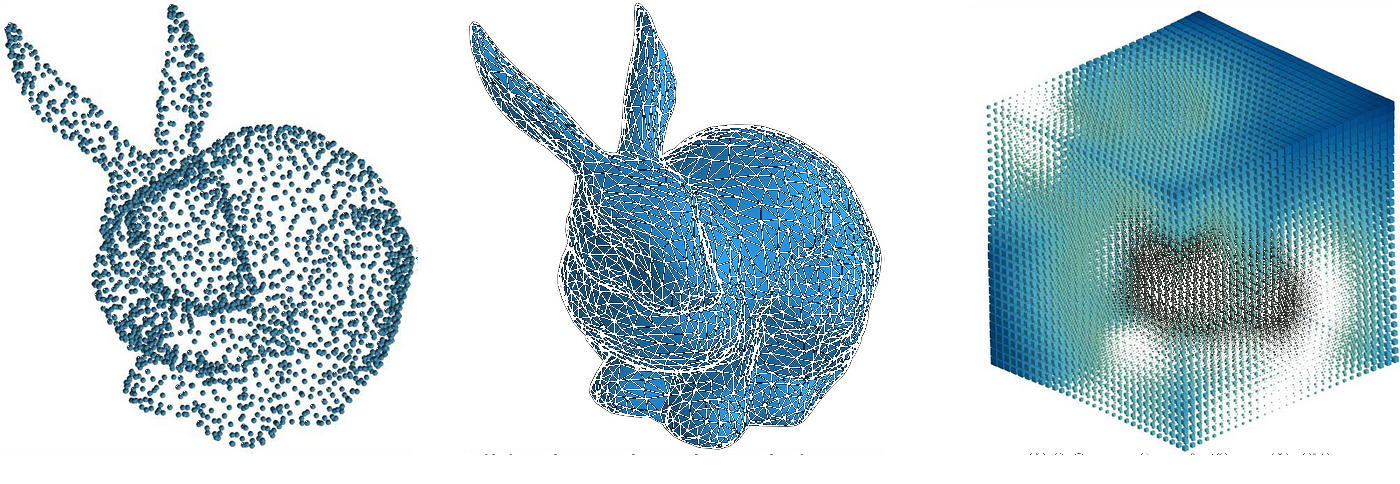
\includegraphics[width=0.8\linewidth,keepaspectratio]{images/chapter2_img/overall_representation_diff.jpg}
        \caption{Διαφορετικές Μορφές αναπαραστάσεων Γραφικών}
        \label{fig:GraphichRepresentationsTHumbnail}
    \end{figure}
\subsection{Άμεσες/Ρητές Αναπαραστάσεις 3D Γραφικών }
    \subsubsection{3D - Αναπαραστάσεις ως πλέγματα τριγώνων}
    \begin{figure}[!tbh]
    \centering
    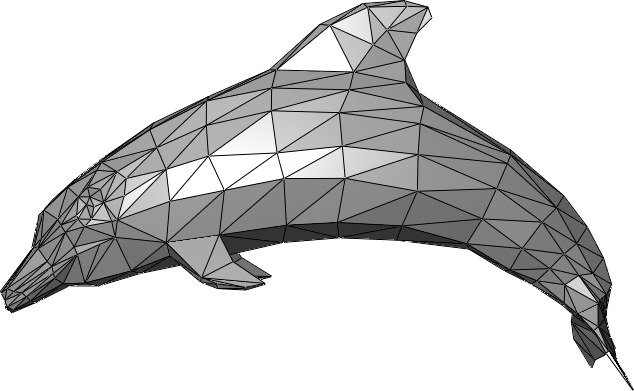
\includegraphics[width=5.5cm]{images/chapter2_img/Dolphin_triangle_mesh.jpg}
    \caption{\enit{3D} πλέγμα τριγώνων που αναπαριστά δελφίνι.}
    \label{fig:1}
    \end{figure} 
\par 
    Στον χώρο της γραφικής υπολογιστών στις περισσότερες περιπτώσεις οποιοδήποτε γραφικό στοιχείο έχει ως δομική μονάδα αναπαράστασης τα κυρτά πολύγωνα. Αυτό, ονομάζεται ρητή αναπαράσταση γραφικών(\enit{explicit representation}). Η συγκεκριμένη τακτική ακολουθείται, καθώς η κυρτότητα του σχήματος δίνει την δυνατότητα διάκρισης του χώρου του οποίο καταλαμβάνει και κατά συνέπεια αυτό βοηθάει σε αλγορίθμους σκίασης. Οι αλγόριθμοι σκίασης, απαιτούν την επίγνωση των ορίων κάθε στοιχειώδους επιφάνειας για τον χρωματισμό της. Κατά σύμβαση η συνηθέστερη επιλογή κυρτού πολυγώνου είναι το τρίγωνο χάρη στα πλεονεκτήματα της απλότητας ως προς αναπαράσταση.
\par 
    Πλειάδες αυτών των κυρτών πολυγώνων (\enit{Triangular Meshes}), αναπαριστούν \enit{3D} μοντέλα και σκηνές του χώρου και κατά συνέπεια κάθε κυρτό πολύγωνο έχει μια τιμή χρώματος που του έχει αποδοθεί από τον αλγόριθμο σκίασης.Για να γίνει αυτό στον \enit{3D} χώρο, αυτός διαμερίζεται σε ογκομετρικό πλέγμα (\enit{Voxel Grid}).
\par 
    Παρόμοιες αναπαραστάσεις στον \enit{3D} χώρο είναι και τα νέφη σημείων \enit{Point Clouds}, τα οποία ωστόσο δεν είναι ιδανικές αναπαραστάσεις στερεών αντικειμένων ή ρευστών (είναι μη συνεχείς και μη πραγματικές συναρτήσεις). Συνήθως χρησιμοποιούνται σε ογκομετρικά δεδομένα και πεδία πυκνότητας (γραφικά σύννεφων) όπου δεν απαιτούνται αναπαραστάσεις συμπαγών επιφανειών.   
\par
    Για τον υπολογισμό του χρώματος σε τέτοιες δομές, απαιτείται τόσο από την υφή αλλά και ο φωτισμός του αντικειμένου. Κατά συνέπεια όλες οι ρητές αναπαραστάσεις γραφικών πριν την προβολή τους, είναι πίνακες που αναπαριστούν τρισδιάστατα ογκομετρικά πλέγματα. Κατά την διαδικασία της απόδοσης που θα αναλυθεί στην συνέχεια είτε με την μέθοδο της ραστεροποίησης(\enit{rasterization}) με χρήση κλασσικών μοντέλων φωτισμού ή χρησιμοποιώντας και μεθόδους ολικού φωτισμού με την μέθοδο ρίψης ακτίνων (\enit{ray tracing, ray casting}) αποτυπώνονται στην οθόνη με δισδιάστατη μορφή. Στα σύγχρονα συστήματα απόδοσης γραφικών (πχ. \enit{Blender, Meshlab} κτλ.) ο χρήστης έχει τη δυνατότητα να δει προοπτικές προβολές του 3D μοντέλου του σε ένα συνεχές χώρο διάφορων οπτικών γωνιών μέσα από το viewport(\textit{επεξεργάσιμος καμβάς γραφικών που χρησιμοποιείται από τον σχεδιαστή}), μετακινώντας την θέση της εικονικής πλέον κάμερας. 


\subsection{Παραμετρικές Αναπαραστάσεις Γραφικών}
\par
    Πέραν των άμεσων αναπαραστάσεων γραφικών που είναι ο κατ' εξοχήν τρόπος με τον οποίο αναπαριστώνται τα στατικά γραφικά στην συντριπτική τους πλειοψηφία, σε διάφορες εφαρμογές, κυρίως στον τομέα της σχεδίασης CAD, χρησιμοποιούνται μαθηματικές αναπαραστάσεις που υπάγονται στην κατηγορία των παραμετρικών αναπαραστάσεων γραφικών. Αυτές οι μορφές γραφικών αναπαραστάσεων μπορεί να γίνουν αρκετά σύνθετες και βασίζονται σε γνωστές συναρτήσεις.

    Πιο συγκεκριμένα, η τεχνική που ακολουθείται είναι η τμηματική προσέγγιση καμπυλών ή επιφανειών, μέσω συναρτήσεων που ονομάζονται πολυώνυμα βάσης \cite{winkel2001generalized}. Ανάλογα τον βαθμό του πολυωνύμου περιγράφονται αντίστοιχης διάστασης γεωμετρικοί τόποι. 

    Σε αυτή την κατηγορία μεθόδων η θέση τυχαίου σημείου $P \in \mathbb{R}^{n}$  προσεγγίζεται από μία διανυσματική συνάρτηση $\mathbf{P(\tau)}$ παραμετροποιημένη ως προς την μεταβλητή $\tau$. Η εν λόγω συνάρτηση, παριστάνεται ως ανάπτυγμα σε ένα πεπερασμένο σύνολο συναρτήσεων βάσης με συντελεστές του αναπτύγματος να αποτελούν μια πλειάδα σημείων του χώρου (τρισδιάστατος χώρος ή δισδιάστατο επίπεδο), που αποκαλούνται σημεία ελέγχου κάτι το οποίο εισάγει και το πρόβλημα των βαθμών ελευθερίας.

    Η βασική μορφή της συνάρτησης $\mathbf{P(\tau)}$ για τα αναπτύγματα σε συναρτήσεις βάσης είναι η ακόλουθη:
    \begin{equation}
        \mathbf{P(\tau)} = \sum_{n=0}^{n} p_i*\phi_i(\tau),
        \label{eq:PolynomialBaseSeries}
    \end{equation}
    
    δηλαδή το άθροισμα πεπερασμένου πλήθους συναρτήσεων βάσης $\phi$ σε $n+1$ σημεία ελέγχου. Προφανώς η έκφραση \ref{eq:PolynomialBaseSeries} μπορεί να χρησιμοποιηθεί με ποικίλα πολυώνυμα, ωστόσο υπάρχουν ορισμένες οικογένειες πολυωνύμων, οι οποίες έχουν επικρατήσει λόγω χρήσιμων ιδιοτήτων τους στην περιγραφή μεγάλου συνόλου γραφικών αναπαραστάσεων. Περισσότερα για τα πολυώνυμα βάσης στο Παράρτημα Κ.\ref{chapter:appendix}.
    
\par    
    Παρά την αναλυτικότητα αυτών των μορφών αναπαράστασης υπάρχουν σημαντικά μειονεκτήματα. Παράδειγμα, η διακριτή και αναγκαία παραμετροποίηση τους αλλά και η αδυναμία περιγραφής τους από συναρτήσεις που μπορούν να αναπαρασταθούν από νευρωνικά δίκτυα. Συνεπώς, δεν αποτελούν κατάλληλη επιλογή ως μέσο αποτύπωσης επιφανειών που βελτιώνει τις παραμέτρους του ώστε να καταφέρει να μάθει την γεωμετρία άγνωστης επιφάνειας (εφόσον δεν είναι εύκολα εκπαδεύσιμες μορφές), μιας και οι παράγωγοι τους σε ορισμένες περιπτώσεις είναι ήδη αρκετά μεγάλου βαθμού και υπάρχει ήδη πεπερασμένος βαθμός ελευθερίας λόγω των σημείων ελέγχου \cite{winkel2001generalized}.
\subsection{Έμμεσες αναπαραστάσεις Γραφικών}
\par
    Οι άμεσες αναπαραστάσεις αυξάνουν το υπολογιστικό κόστος των αλγορίθμων καθώς είναι ακατέργαστες μορφές ενώ οι  παραμετρικές είναι δύσκολες στην βελτιστοποίηση. Σε αυτό το πρόβλημα, δίνουν λύση οι έμμεσες αναπαραστάσεις δηλαδή η περιγραφή των σημείων του χώρου για παράδειγμα μέσα από την απόστασή του από την επιθυμητή επιφάνεια. Έτσι, για παράδειγμα, η επιφάνεια είναι το σύνολο των σημείων που δίνουν μηδέν για αυτήν την συνάρτηση απόστασης.
\par 
    Αυτές οι αναπαραστάσεις, έχουν πλήθος πλεονεκτημάτων με βασικότερο όλων ότι μπορούν να περιγραφούν μέσω νευρωνικών δικτύων, μιας και ένα νευρωνικό δίκτυο ουσιαστικά περιγράφει σύνολα επιπέδων(πολλαπλότητες \ref{theorem: Bocher's Theorem} , απόδειξη \ref{chapter:appendix}). Έτσι, με κατάλληλες παραμέτρους και έλεγχο της επιθυμητής εξόδου ένα δίκτυο μπορεί να προσεγγίσει έμμεσα μια τρισδιάστατη επιφάνεια προσεγγίζοντας την συνάρτησή προσημασμένης απόστασης. Έτσι προσεγγίζει μια πολύ πιο ευέλικτη δομή αυτή των οριακών πολλαπλοτήτων ή πιο συγκεκριμένα της συνάρτησης που αναπαριστά ισομετρική επιφάνεια για συγκεκριμένη τιμή.
    \begin{figure}[H]
    \begin{subfigure}{.47\textwidth}
        \centering
        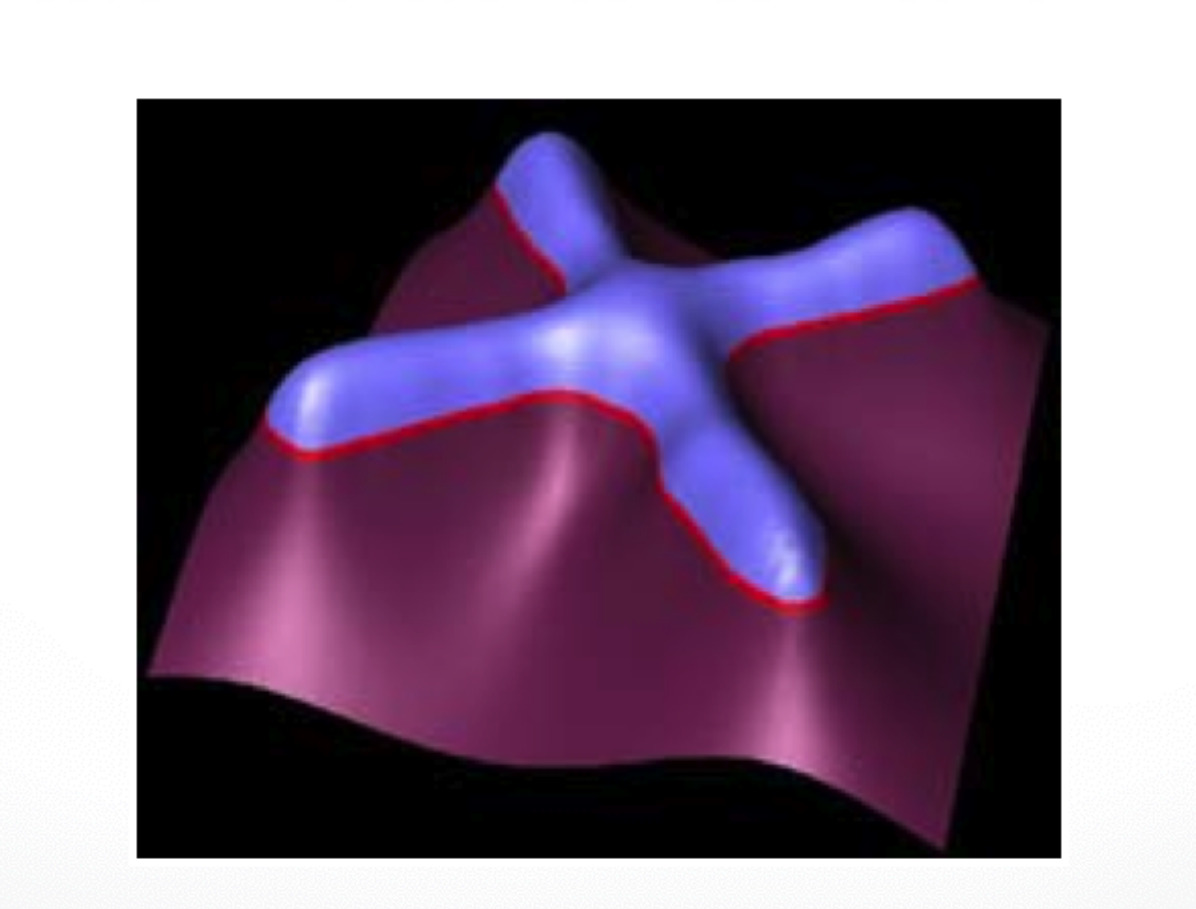
\includegraphics[width=.5\textwidth]{images/chapter2_img/levelSetOf2DDefines1dline.jpg}\\
        \small{Πολλαπλότητες δύο διαστάσεων ορίζουν καμπύλη μιας διάστασης}
    \end{subfigure}
    \hfill
    \begin{subfigure}{.47\textwidth}
        \centering
        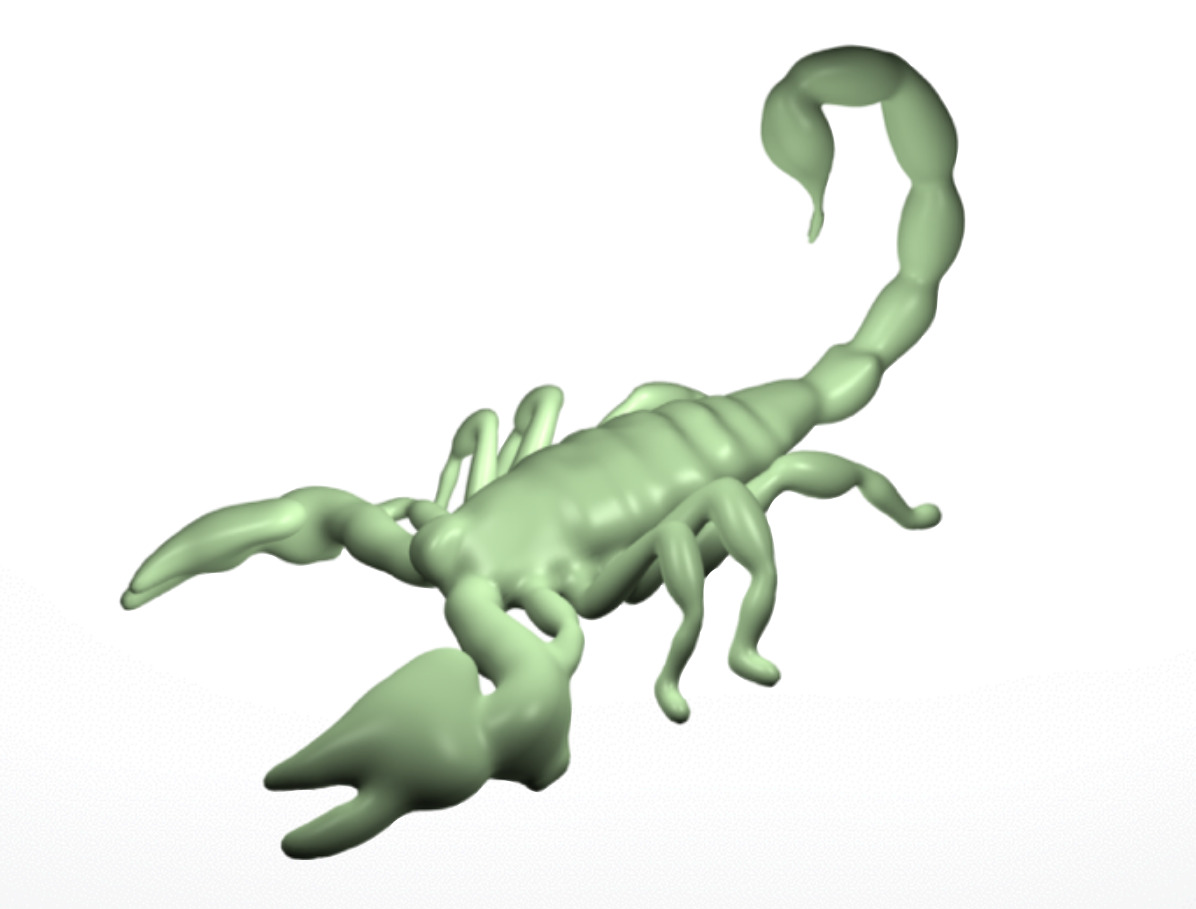
\includegraphics[width=.5\textwidth]{images/chapter2_img/levelSetOf3DDefines2dSuraface.jpg}\\
        \small{Πολλαπλότητες τριών διαστάσεων ορίζουν έμμεσα επιφάνεια σκορπιού}
    \end{subfigure}
    \caption{Πολλαπλότητες ορίζουν έμμεσα ισομετρικές επιφάνειες χαμηλότερης διάστασης σε όριο απόφασης}
    \end{figure}
\clearpage
\par 
    Μια γενική μορφή έμμεσης συνάρτησης ορίζεται ως εξής:
    \begin{itemize}
        \item Εσωτερικά Σύνολα Επιπέδων: $F(x, y, z)<0$
        \item Εξωτερικά Σύνολα Επιπέδων: $F(x, y, z)>0$
        \item Οριακή Επιφάνεια: $F(x, y, z)=0$
    \end{itemize}
    Σκοπός είναι η επιτυχής περιγραφή της οριακής επιφάνειας.
    Σε κάθε περίπτωση, η κλίση $\nabla{F}$ είναι ορθογώνια στα σύνολα επιπέδων (εφόσον ταυτίζεται με το κάθετο διάνυσμα στο εφαπτόμενο επίπεδο) και ειδικότερα στην περίπτωση που η έμμεση επιφάνεια περιγράφεται από συνάρτηση προσημασμένης απόστασης (\(sign \in \{-1,1\}\), το $|\nabla F| = 1$. Εφόσον αυτού του είδους οι έμμεσες συναρτήσεις ή πεδία χρησιμοποιούνται για να περιγράψουν την γεωμετρία των εκπαιδευόμενων επιφανειών, γίνεται  περισσότερη ανάλυση στο κεφάλαιο \ref{section:sdf}. \\
\par    
    Ταυτόχρονα, υπάρχουν και άλλες μορφές έμμεσων αναπαραστάσεων γραφικών όπως είναι τα οκταδικά δέντρα \cite{hearn2011computer} ή καλύτερα octrees τα οποία θεωρούνται δομές που αναπαριστούν την κάλυψη ενός ογκομετρικού στοιχείου (voxel) από σημεία. Έτσι,  τα οκταδικά δέντρα χρησιμοποιούνται συχνότερα για τη διαίρεση ενός τρισδιάστατου χώρου διαιρώντας τον αναδρομικά σε \(n\) οκτάδες\footnote{(όπου n αφορά την ανάλυση)} και περιγράφουν σε ποιες περιοχές υπάρχουν σημεία. Αυτή η δομή, χρησιμοποιεί την a-priori ιδιότητα της συνοχής του χώρου για να ελαττώσει τις αποθηκευτικές απαιτήσεις των τρισδιάστατων αντικειμένων και επίσης παρέχει μια βολική περιγραφή για την αποθήκευση πληροφορίας σχετικά με το εσωτερικό των αντικειμένων. Ωστόσο, δεν αποτελεί κατ' εξοχήν συνεχή μορφή αναπαράστασης που σημαίνει ότι χωλαίνει στην αναπαράσταση συμπαγών επιφανειών υψηλής λεπτομέρειας. Παρακάτω φαίνεται ένα παράδειγμα οκταδικού δέντρου και πως δίνει πληροφορία για τρισδιάστατα δεδομένα. 
    \begin{figure}[H]
        \centering
        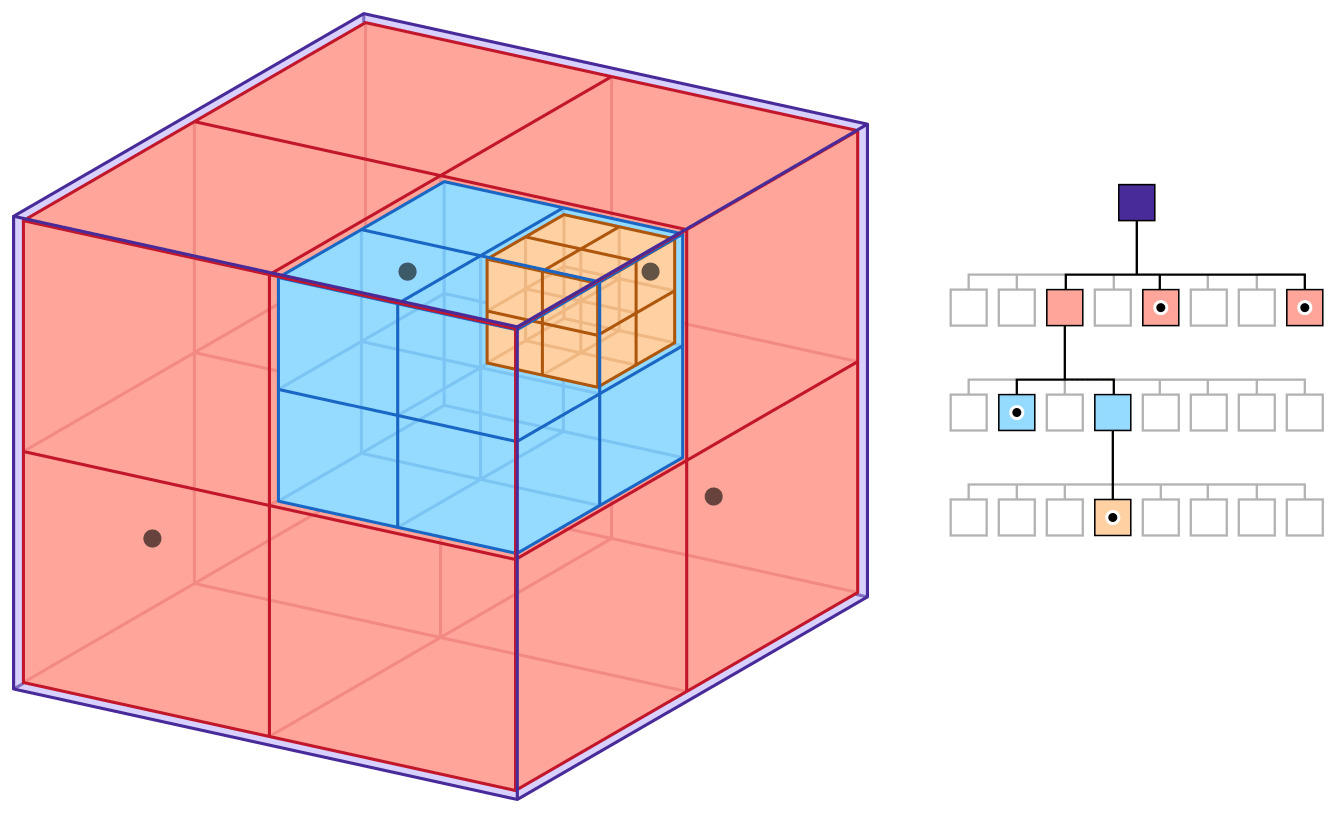
\includegraphics[width=.8\linewidth]{images/chapter2_img/octree.jpg}
        \caption{Οκταδικό Δέντρο}
        \label{fig:octree}
    \end{figure}
    \clearpage
\par 
    Συνοψίζοντας, γίνεται επιλογή έμμεσων επιφανειών για αναπαράσταση 3D δομών λόγων των πλεονεκτημάτων που αναφέρθηκαν και φαίνονται συνοπτικά στην παρακάτω εικόνα :\\
    \begin{figure}[H]
        \centering
        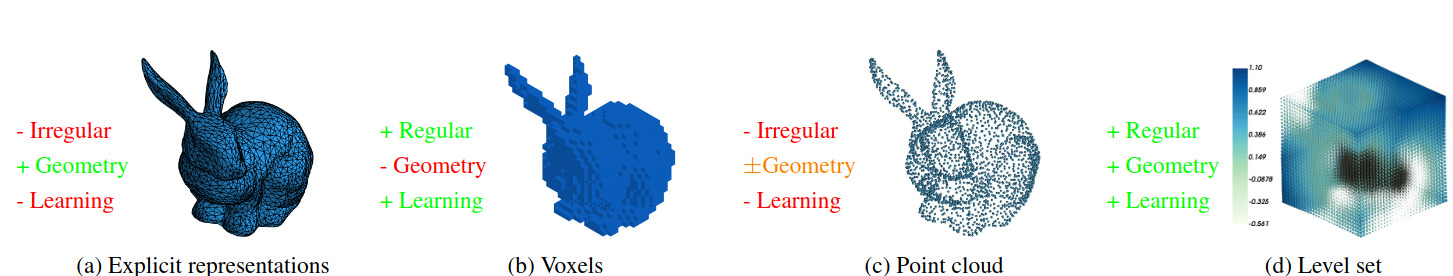
\includegraphics[width=\linewidth,keepaspectratio]{images/chapter2_img/TrainabillityOfGraphicsRepresentations.jpg}
        \caption{Πλεονεκτήματα και μειονεκτήματα Γραφικών Αναπαραστάσεων (Πηγή \cite{michalkiewicz2019implicit})}
        \label{fig:RepresentationsAdsDis}
    \end{figure}
\par
    Ο τρόπος εξαγωγής πλεγμάτων τριγώνων (τυπική μορφή αποθήκευσης τρισδιάστατων δεδομένων) από έμμεση αναπαράσταση επιφάνειας είναι αρκετά ενδιαφέρων με έναν από τους κλασσικούς πλέον αλγορίθμους την γραφική  υπολογιστών να αποτελεί τον αλγόριθμο \enit{contouring} (περιγράμματος) Marching Cubes, ο οποίος αφήνεται στο παράρτημα Κεφ.\ref{chapter:appendix} για τον αναγνώστη.
